Se procede a mostrar los valores de campo magnético $B$ obtenidos en distintas posiciones del cilindro para los valores
de resistencia que minimizan la variación de dicho campo en la Figura \ref{fig:variacion_campo}. Se obtuvo una variación del 2,03\% entre $\SI{15,0\pm0,1}{\centi\meter}$ y $\SI{45,0\pm0,1}{\centi\meter},$
la que será la zona de trabajo del tubo.

\begin{figure}[H]
    \centering
    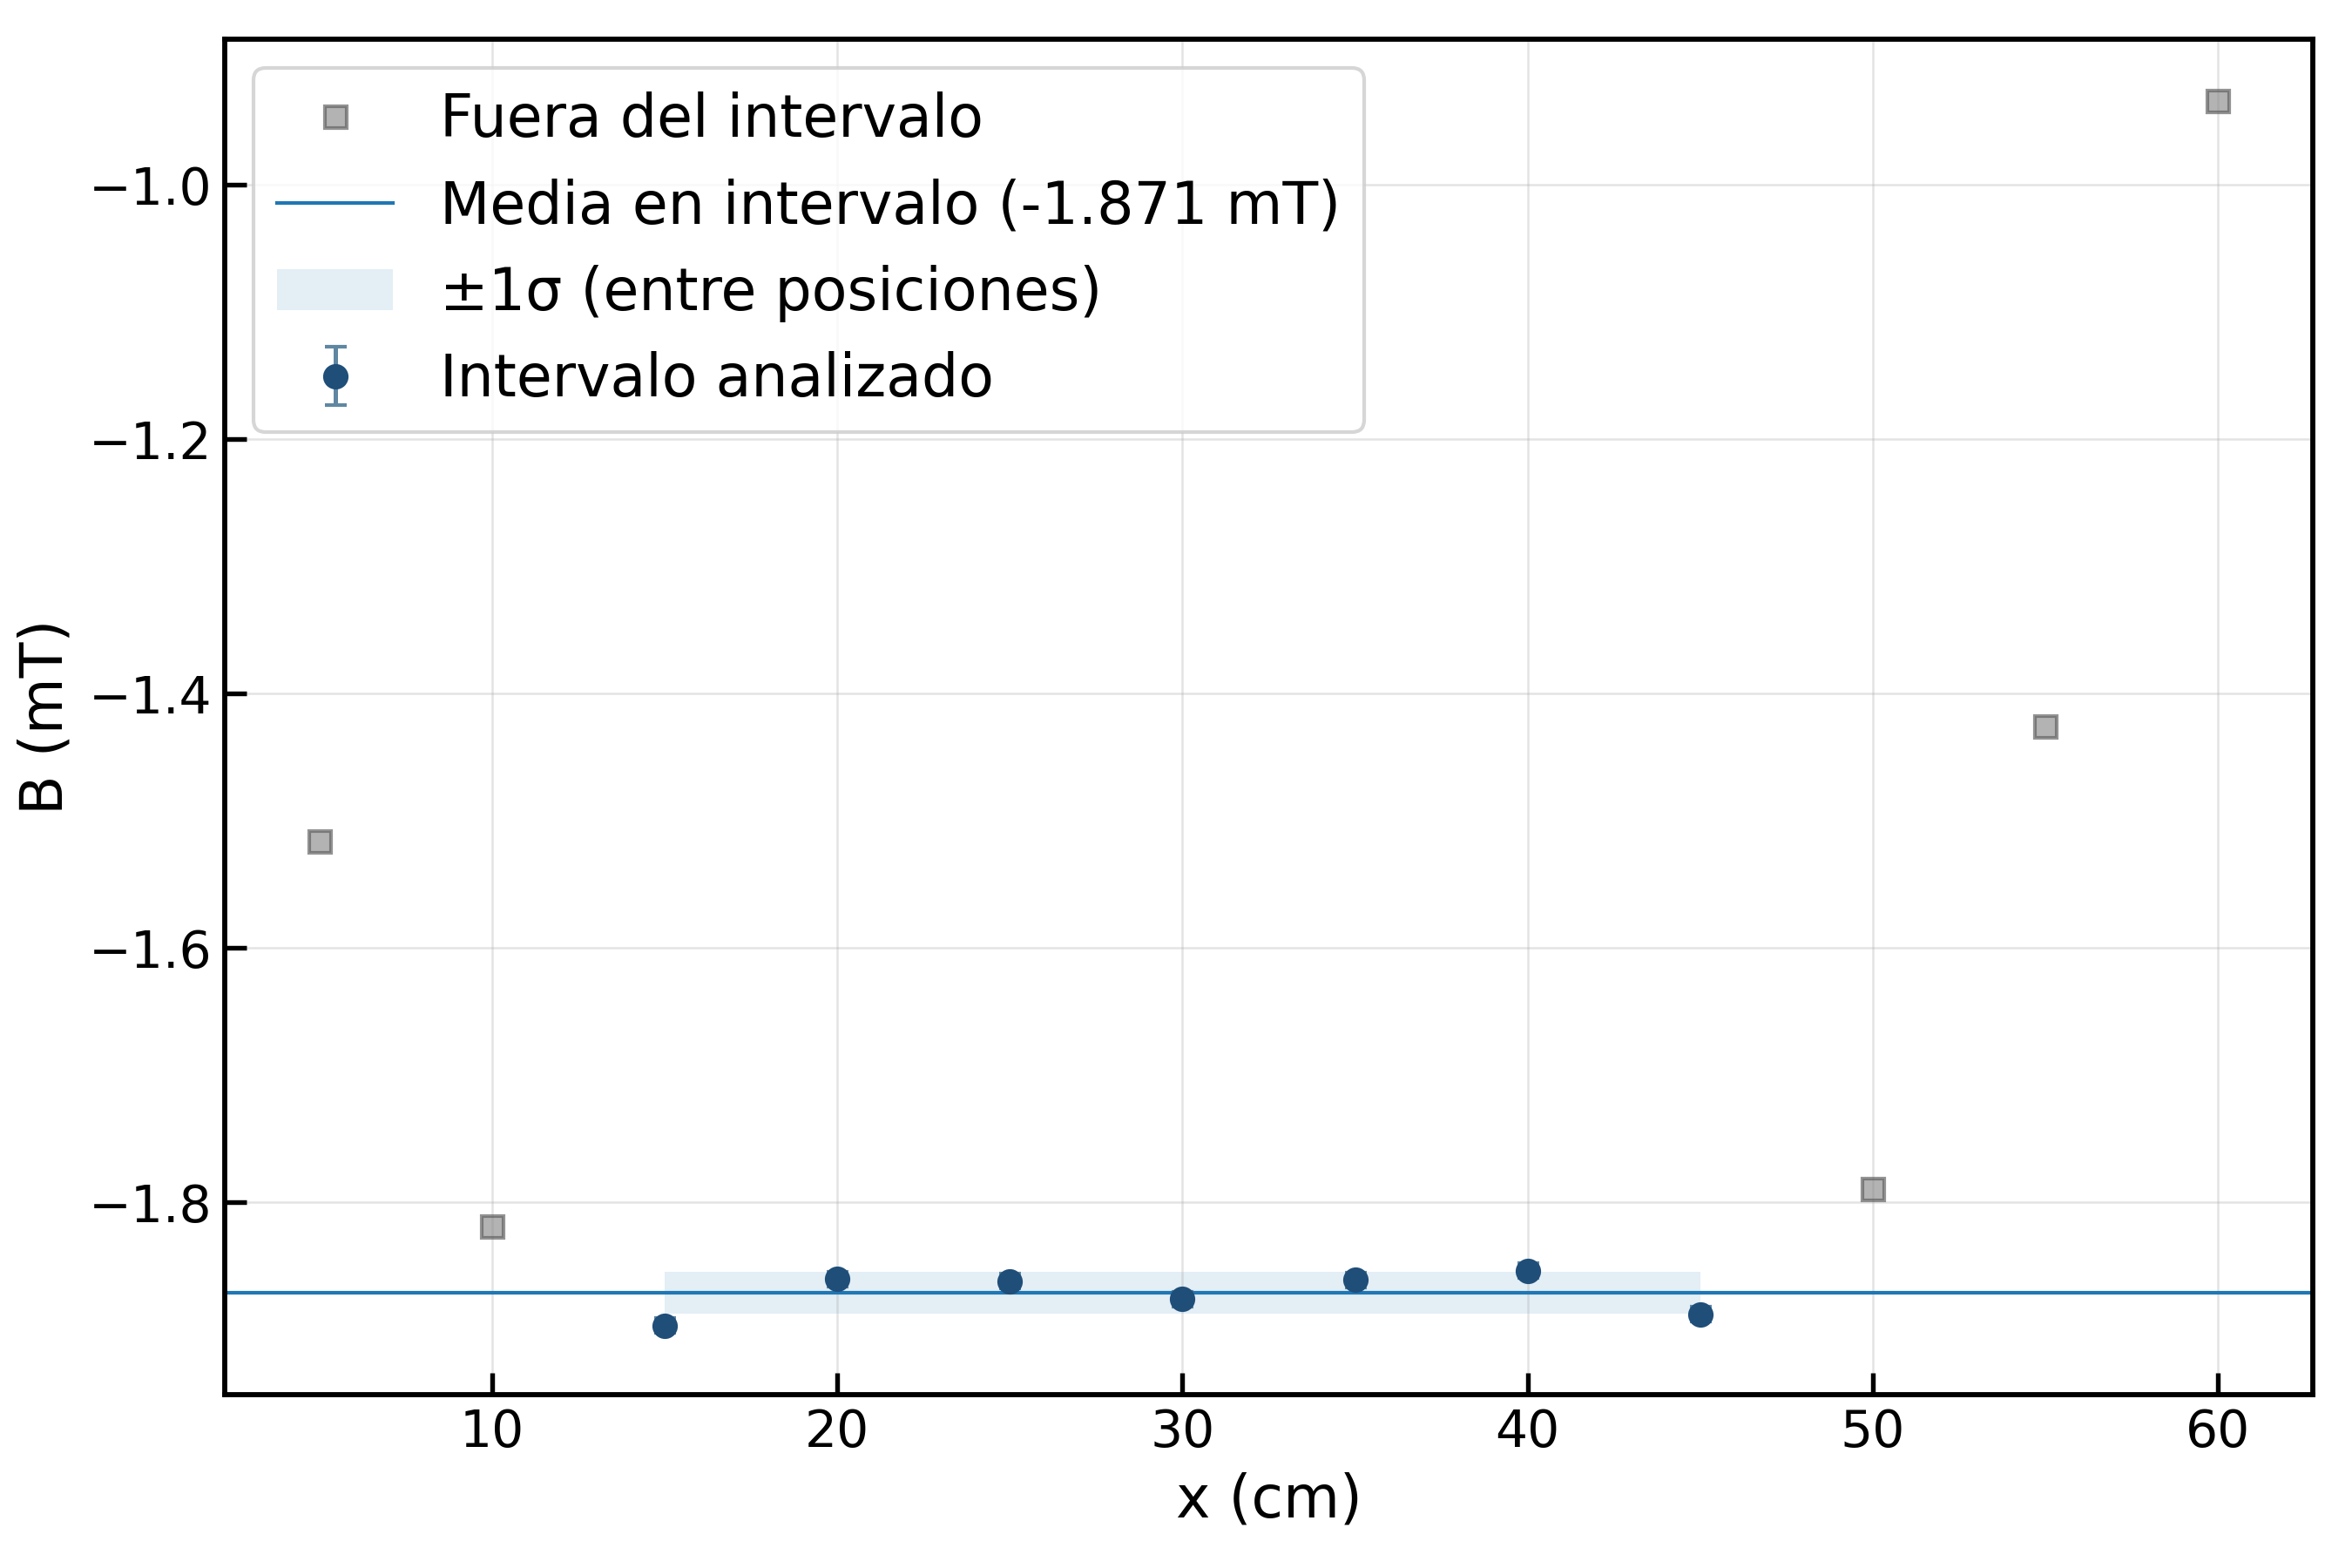
\includegraphics[width=0.49\textwidth]{Images/B_vs_x_mT.png}
    \caption{Campo magnético $B$ en función de la posición $x$ a lo largo del cilindro para $I=\SI{3,00\pm0,03}{\ampere}$.}
    \label{fig:variacion_campo}
\end{figure}

Una vez readaptado el armado experimental, se procedió a encontrar los mínimos relativos de área de impacto de electrones
para distintos valores de tensión de aceleración $V.$ Se muestra en la Figura \ref{fig:area_impacto} como la variación de tensión de alimentación (y por tanto de campo magnético)
afecta al área relativa de impacto para una misma tensión de aceleración.

\begin{figure}[h]
    \centering

    \begin{subfigure}[b]{0.48\columnwidth}
        \centering
        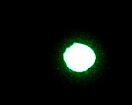
\includegraphics[width=\linewidth]{Images/roi_20260302_162848_V0.016.png}
        \caption{Área de impacto para un bajo valor de $B.$}
        \label{fig:subfig1}
    \end{subfigure}
    \hfill
    \begin{subfigure}[b]{0.48\columnwidth}
        \centering
        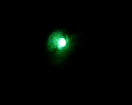
\includegraphics[width=\linewidth]{Images/roi_20260302_163106_V0.062.png}
        \caption{Área de impacto para un alto valor de $B.$}
        \label{fig:subfig2}
    \end{subfigure}

    \caption{Imágenes capturadas por la cámara digital para distintos valores de $B$
    a una tensión de aceleración de $V=\SI{700,00\pm0,05}{\volt}$.}
    \label{fig:area_impacto}
\end{figure}

Para cada valor de tensión de aceleración, se gráfico el área relativa en función de la tensión de alimentación,
a modo de encontrar los mínimos relativos de área relativa. Esto se muestra en la Figura \ref{fig:area_vs_V}.

\begin{figure}[h]
    \centering
    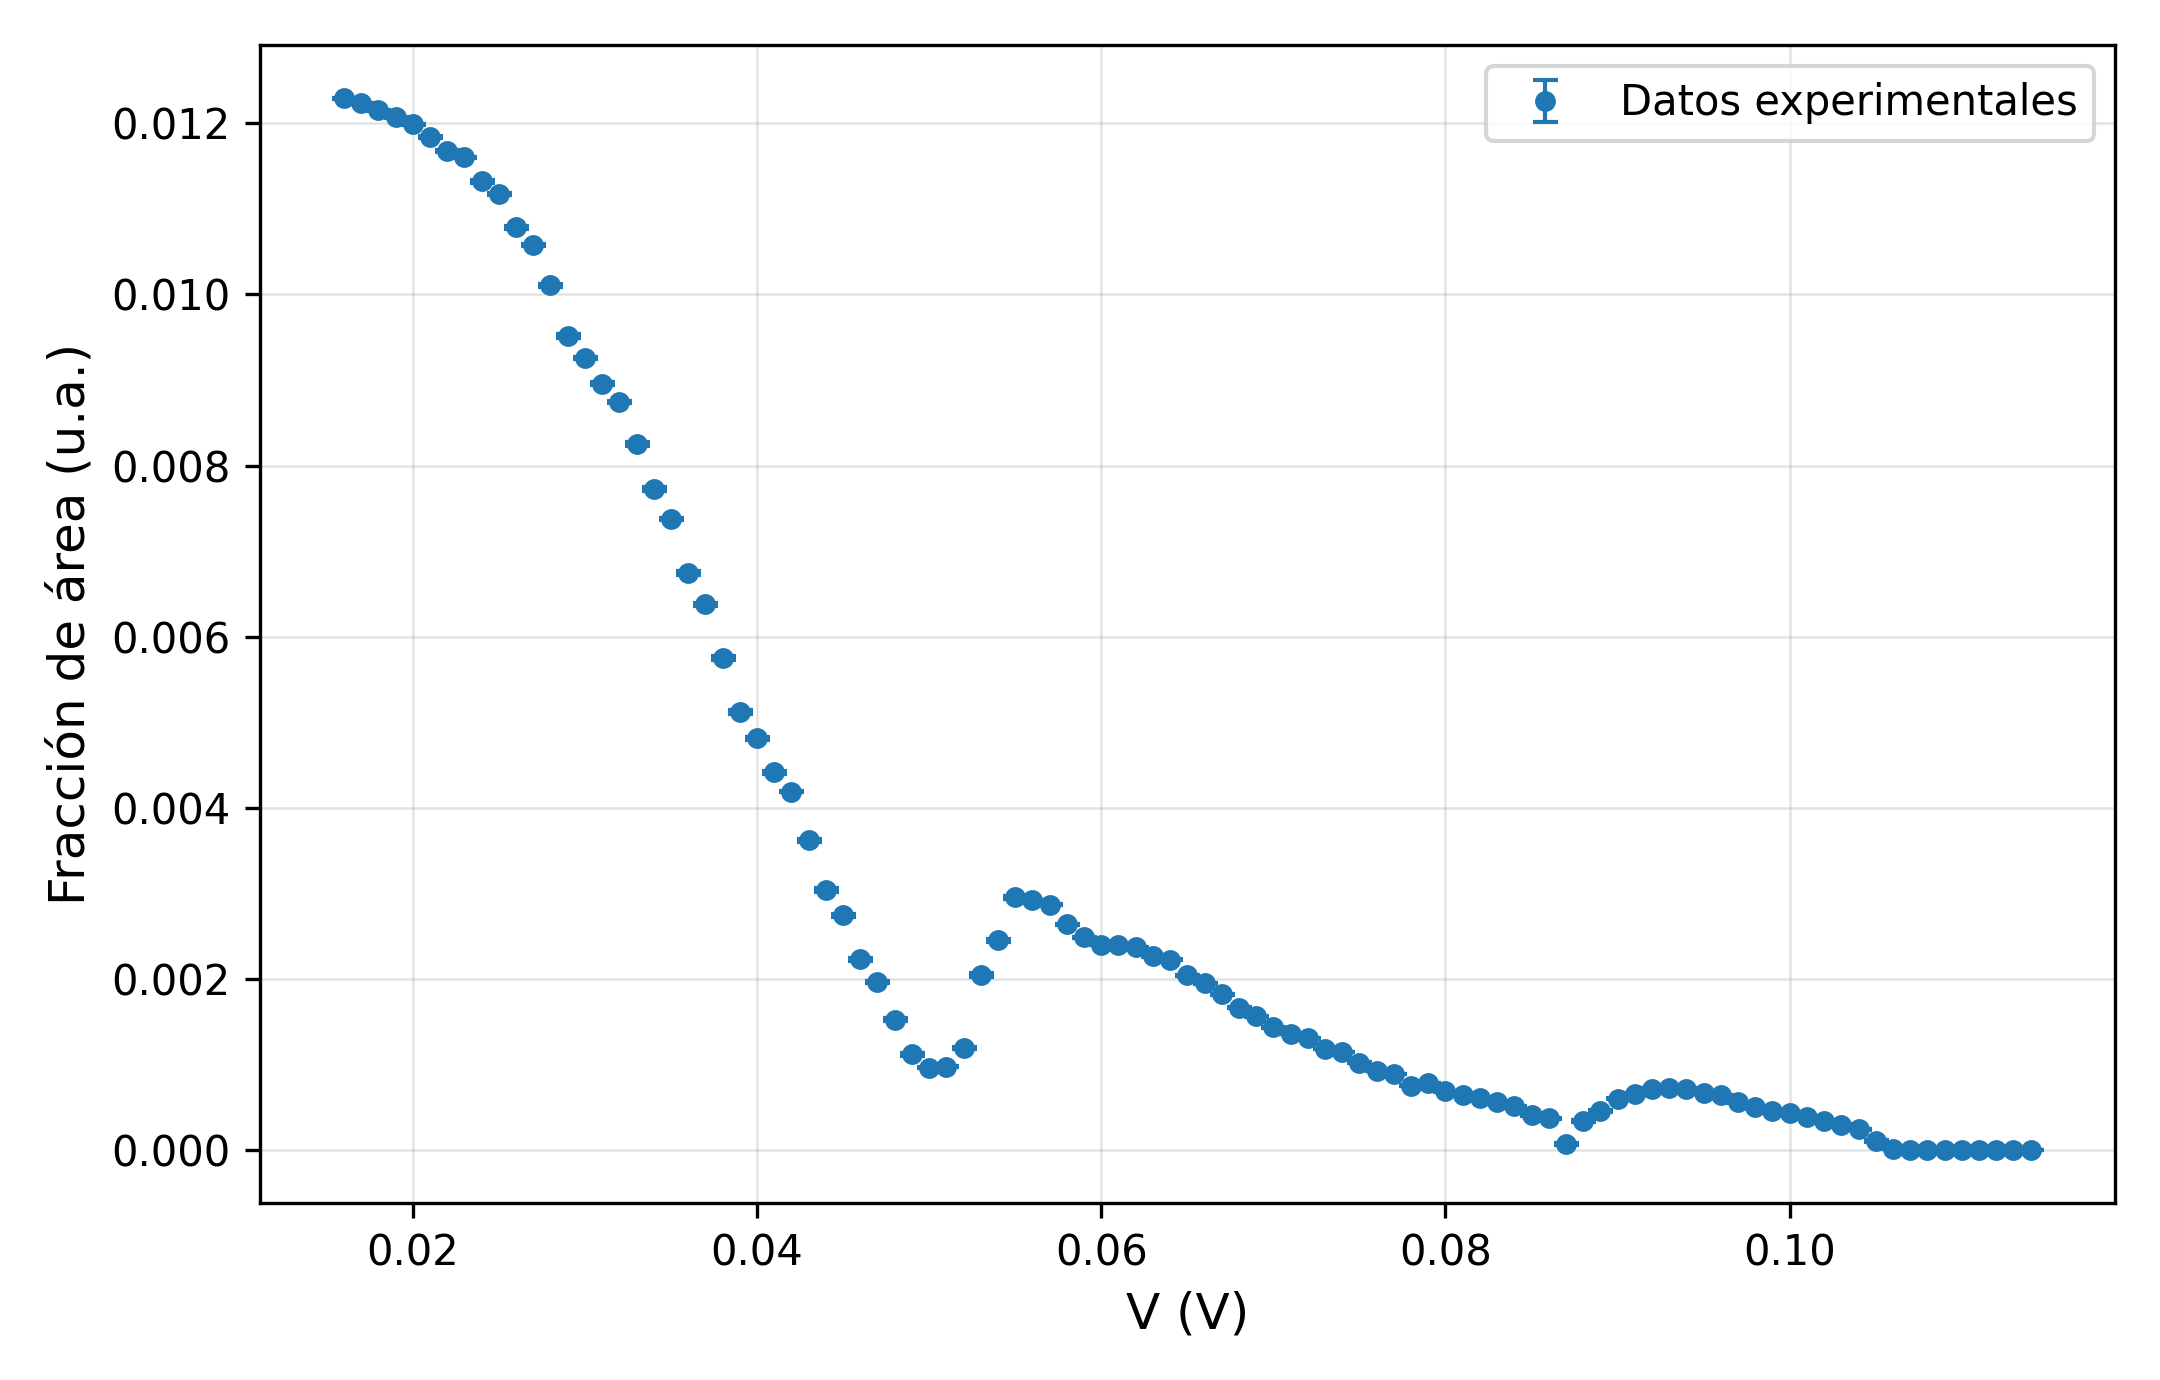
\includegraphics[width=\columnwidth]{Images/frac_vs_V.png}
    \caption{Área relativa de impacto en función de la tensión de alimentación para una tensión de aceleración $V=\SI{500,00\pm0,05}{\volt}$.}
    \label{fig:area_vs_V}
\end{figure}

Se observa una curva similar a la esperada por la Ecuación PONER ECUACION CORRESPONDIENTE, aunque esto no fue así
para otros valores de tensión de aceleración. El por qué de esto se discutirá más adelante.

Luego, mediante un script de Python, se encontraron los mínimos
relativos de área relativa, identificándose además el orden de cada mínimo. Dichos mínimos se muestran en la Figura \ref{fig:minimos}:

\begin{figure}[h]
    \centering
    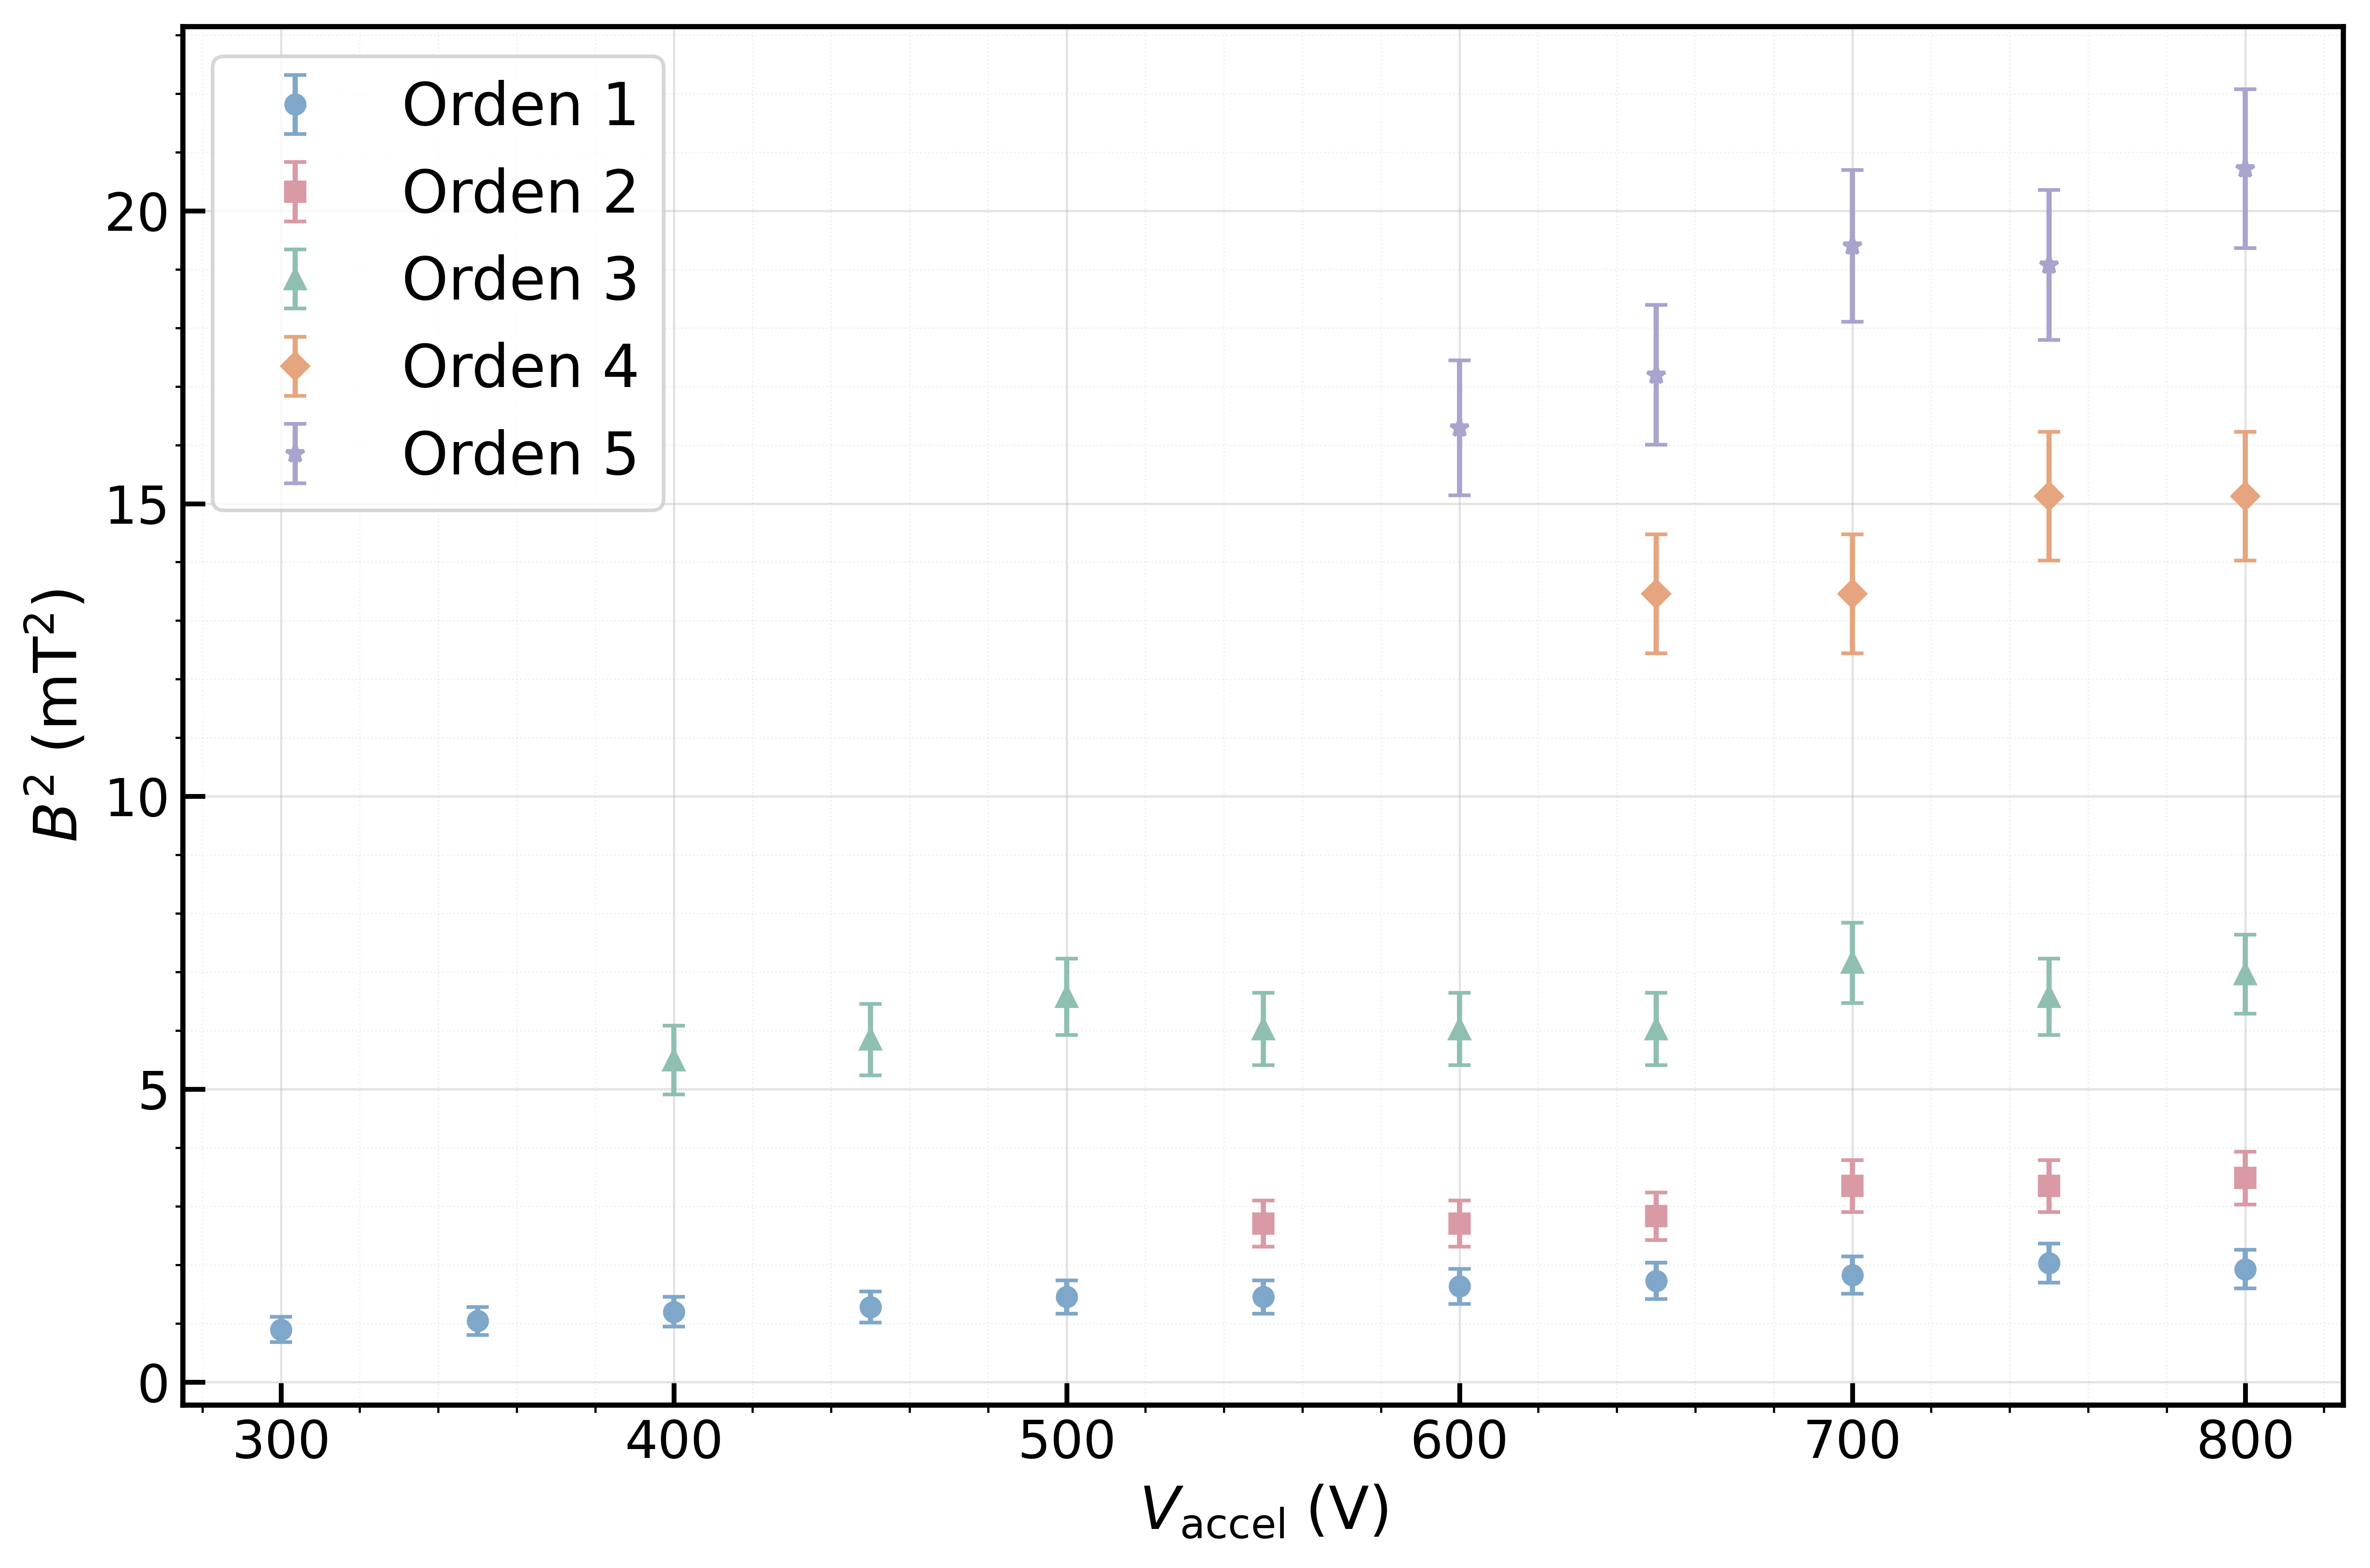
\includegraphics[width=\columnwidth]{Images/Datos BV.png}
    \caption{Valores de campo magnético $B$ que minimizan el área relativa en función de la tensión de aceleración $V.$}
    \label{fig:minimos}
\end{figure}

Para cada orden de mínimos, la relación debería ser lineal, pero se observa que solo algunos ordenes cumplen esto, lo que es inconsistente
con la teoría. Luego se procedió a normalizar por $n^2$, ya que dicha relación debería ser lineal y se realizó un ajuste de dichos datos. Esto se muestra en la Figura \ref{fig:minimos_normalizados}:

\begin{figure}[h]
    \centering
    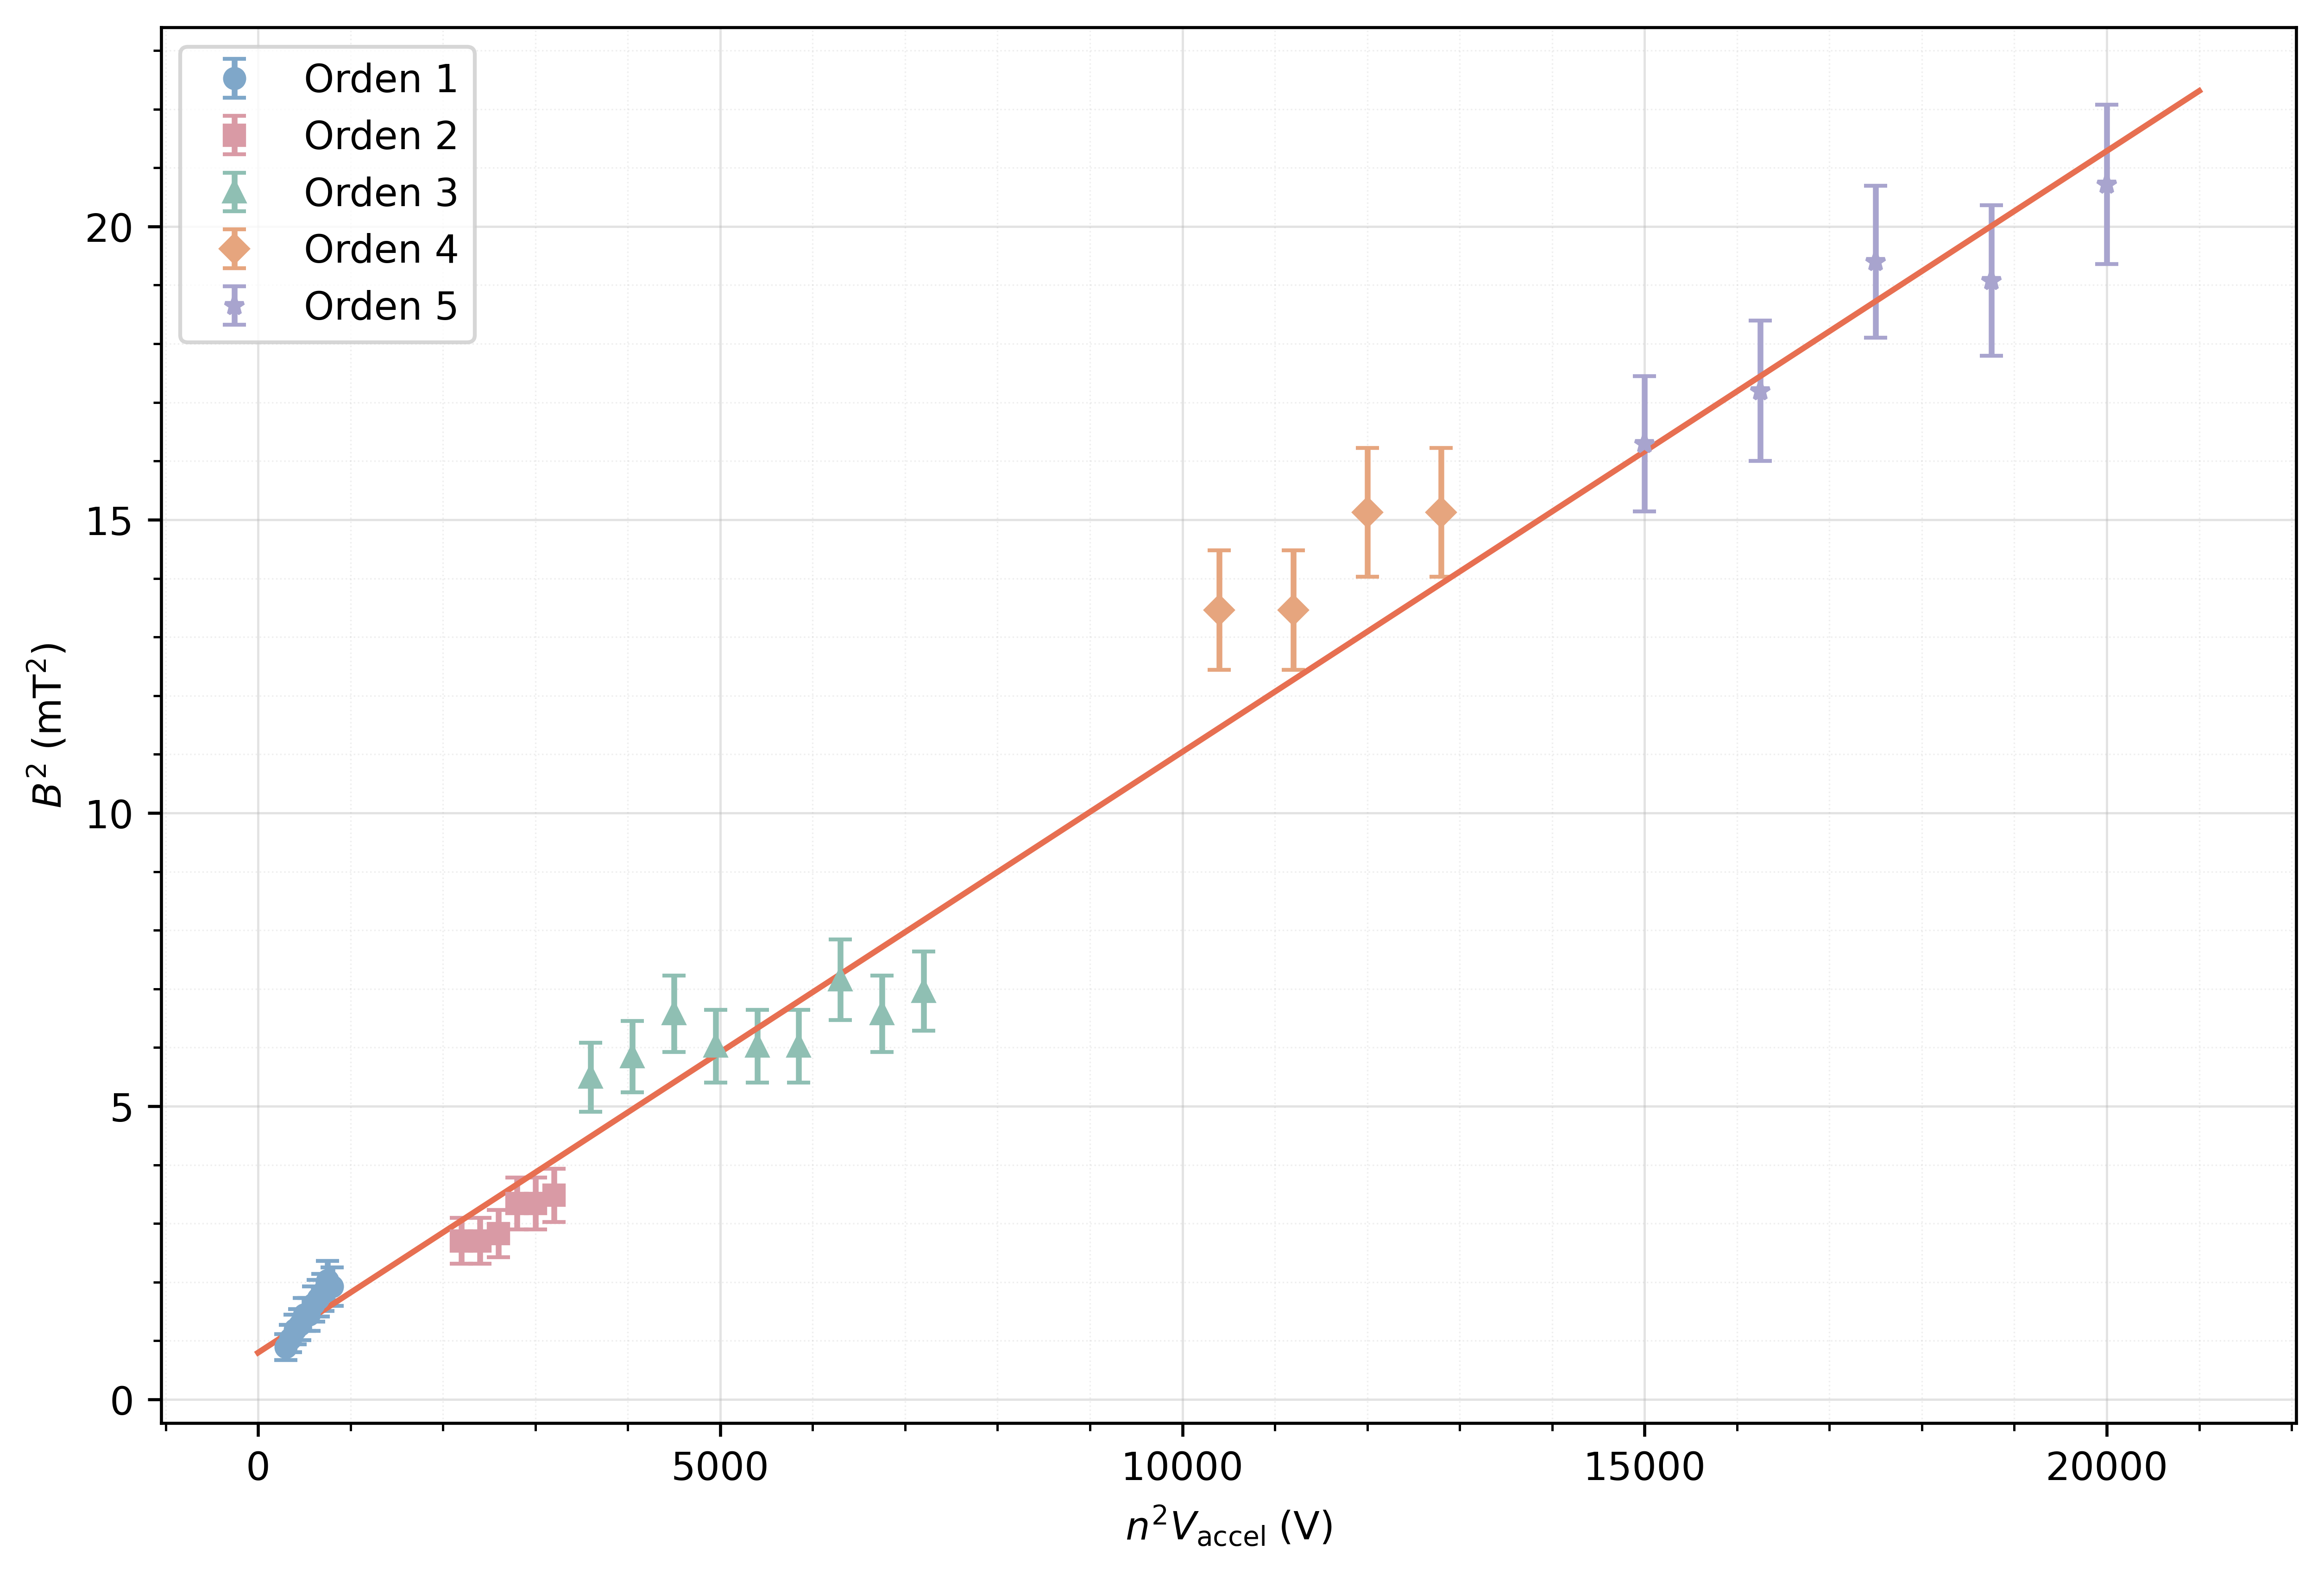
\includegraphics[width=\columnwidth]{Images/Ajuste_Bn2V.png}
    \caption{Valores de campo magnético $B$ que minimizan el área relativa en función de la tensión de aceleración $V,$ normalizados por $n^2,$ junto a su ajuste}
    \label{fig:minimos_normalizados}
\end{figure}

A partir de la pendiente del ajuste y la Ecuación ECUACION QUE HAY QUE PONER, se determinó que la relación
carga-masa del electrón es $e/m=\left( 6,7 \pm 0,4 \right)\times 10^{11}\,\unit{\coulomb\per\kilogram},$ valor lejano al aceptado de $1,75882000838(55)\times 10^{11}\,\unit{\coulomb\per\kilogram}$\cite{nist_em}.

Como en la Figura \ref{fig:minimos_normalizados} se observa que la pendiente de los valores para el primer orden es mayor (y por lo tanto una menor $e/m$), se
hizo un ajuste sobre esos datos únicamente para ver si estos eran más consistentes, pero el valor obtenido fue de $e/m=\left( 3,1 \pm 0,2 \right)\times 10^{11}\,\unit{\coulomb\per\kilogram},$ valor todavía
lejano del aceptado, aunque mejor que el obtenido anteriormente.